\section{overhead}
\jyr{We give a sample result in Figure~\ref{fig:sample}
\begin{figure}
\centering 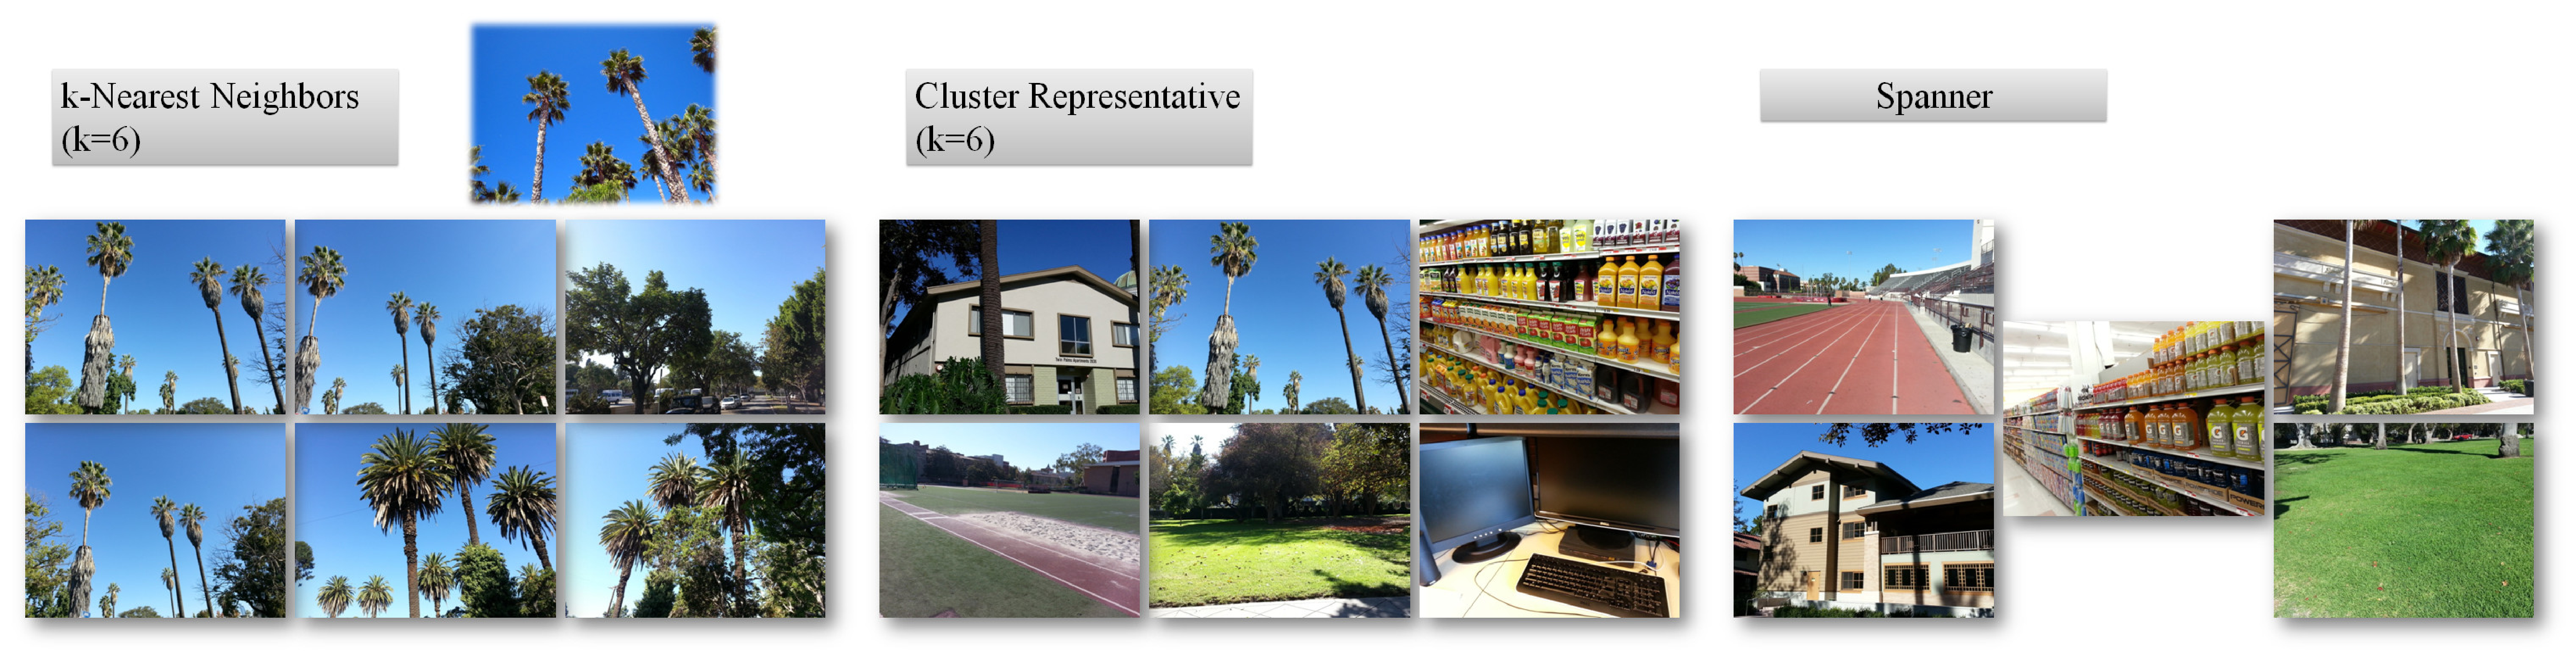
\epsfig{file=pics/sample_query.eps, height=2in}
%\vspace{-1mm}
\caption{ K Cluster Representative  and Spanner Query Sample Result}
\vspace{-6mm}
\label{fig:sample}
\end{figure} 
These photos are taken by two phones, about different scenarios in about 6 different locations: campus, garden, track and field, supermarket, CS lab. We run our $K Cluster Representative$ query and $Spanner$ query on the photo set with  total 175 feature vectors (some from short videos), and results are shown on Figure~\ref{fig:sample}
 }

\subsection{System Overhead}
\label{sec-4-3}

\subsubsection{Metrics}
 
In \mscope, we measure the end-to-end speed from task posting to file uploaded to MSCloudDB, generally the average speed for uploading a  1.5MB or so image is about 466KB/s with WiFi and 408KB/s with ATT 4G in our area. 

We also find that when file size goes larger, the speed increases some. To understand the reason behind this, we measure each component of \mscope that could cause the latency other than the network speed. The results are shown in ~\ref{tab:factor}, 
\begin{table}
    \centering
    \begin{tabular}{ | l | l | l |}
    \hline
    Drawback Factors & Average Latency(ms) \\ \hline
    Server Notification & 231 \\ \hline
    C2DM(send-to-receive) & 251 \\ \hline
    Task Exec & 2103 \\ \hline
    Upload scheduling & 46 \\ \hline
    Server-to-Server File Feteching  & 67 \\ \hline
    \end{tabular}
    \caption{Potential Drawback Factors For uploading Speed}
    \label{tab:factor}
\end{table}
It's  easy to find that major drawback factor is task execution which takes about 2s, other factors such as Server-to-Server Notification as well as C2DM message delay are some other major factors that cause \mscope upload speed performance degrading.


\subsubsection{Results: Overhead}
\label{sec-4-4}
In the end, we measure  the latency of the component in MSCloudQ, the results are show in \ref{tab:overhead}
\begin{table}
    \centering
    \begin{tabular}{ | l | l |}
    \hline
    System Components & Average Latency(ms) \\ \hline
    Query Parse & 612 \\ \hline
    Optimization(Spanner) & 89 \\ \hline
    Optimization(K Clusters) & 52 \\ \hline
    Optimization(Top K) & 11 \\ \hline
    \end{tabular}
    \caption{System Components Overhead}
    \label{tab:overhead}
\end{table}
From the results, one major delay is Query parsing, which we think depends on what script you run in background. Other parts are neglectable.



